                                                                                                           %------------------------------------------------------------------% Cannabis Data Science | Saturday Morning Statistics | 10/30/2021
%
% FIXME: Add bibliography
% https://tex.stackexchange.com/questions/148893/package-biblatex-error-incompatible-package-ucs-begindocument?noredirect=1&lq=1
% https://tex.stackexchange.com/questions/261595/how-to-rerun-biber-on-the-file
% https://tex.stackexchange.com/questions/229638/package-biblatex-warning-babel-polyglossia-detected-but-csquotes-missing
% https://tex.stackexchange.com/questions/49610/use-biblatex-and-utf8
% https://stackoverflow.com/questions/1507672/putting-citation-text-on-same-slide-with-latex-beamer
%------------------------------------------------------------------%
\documentclass[xcolor={dvipsnames}]{beamer}
\hypersetup{pdfpagemode=FullScreen}
\mode<presentation> %TEMPLATE
{ \usetheme{Boadilla}
  \usecolortheme{orchid}
  \usefonttheme{default}
  \setbeamertemplate{navigation symbols}{}
  \setbeamertemplate{caption}[numbered]} 
\usepackage[english]{babel}
\usepackage[utf8x]{inputenc}
\setbeamersize{text margin left=0.5in,text margin right=0.5in}

\usepackage[dvipsnames]{xcolor}
\definecolor{DarkGreen}{RGB}{2, 48, 32}
\definecolor{CalyxGreen}{RGB}{34, 153, 84}
\definecolor{DarkOrange}{RGB}{199, 0, 57}
\definecolor{LightOrange}{RGB}{255, 87, 51}
\definecolor{LightGreen}{RGB}{218, 247, 166}
\definecolor{LightYellow}{RGB}{255, 195, 0}

\setbeamercolor*{palette primary}{bg=LightGreen, fg = DarkGreen}
\setbeamercolor*{palette secondary}{bg=LightGreen, fg=DarkGreen}
\setbeamercolor*{palette tertiary}{bg=LightGreen, fg = DarkGreen}
%\setbeamercolor*{palette quaternary}{bg=myNewColorD, fg = green}

%------------------------------------------------------------------%
% FIXME: Bibliography
%------------------------------------------------------------------%
%\usepackage{csquotes}
%\usepackage[style=verbose]{biblatex}
%\addbibressource{presentation-bib.bib}

%------------------------------------------------------------------%
% Packages
%------------------------------------------------------------------%
\usepackage{amsmath}
\renewcommand*\footnoterule{} %No sperating line on footnote
\usepackage{mathtools} %ANNOTATING EQUATIONS
\usepackage{hhline} %DOUBLBARS
\newcommand\T{\rule{0pt}{2.5ex}} %TOPSTRUT
\newcommand\B{\rule[-1.25ex]{0pt}{0pt}} %BOTTOMSTRUT
\newenvironment<>{varblock}[2][.9\textwidth] %RESIZED BLOCKS
  {\setlength{\textwidth}{#1}
  \begin{actionenv}#3
    \def\insertblocktitle{#2}\par
    \usebeamertemplate{block begin}}
  {\par\usebeamertemplate{block end}
  \end{actionenv}}
\defbeamertemplate{enumerate item}{largeball} %LARGE BALLS
{\begin{pgfpicture}{-1ex}{-0.65ex}{1.5ex}{1.5ex}
\usebeamercolor[fg]{item projected}
{\pgftransformscale{2.5}\pgftext{\Large\pgfuseshading{bigsphere}}}
{\pgftransformshift{\pgfpoint{0pt}{0.5pt}}
\pgftext{\usebeamerfont*{item projected}\small\insertenumlabel}}
\end{pgfpicture}}
\usepackage{tikz} % FANCY ARROWS
\usepackage{xparse}
\NewDocumentCommand\UpArrow{O{2.0ex} O{black}}{%
   \mathrel{\tikz[baseline] \draw [->, line width=0.5pt, #2] (0,0) -- ++(0,#1);}} % FANCY UPARROW
\NewDocumentCommand\DownArrow{O{2.0ex} O{black}}{%
   \mathrel{\tikz[baseline] \draw [<-, line width=0.5pt, #2] (0,0) -- ++(0,#1);}} % FANCY DOWNARROW
%\vskip 1cm
\makeatletter
\newcommand{\LeftEqNo}{\let\veqno\@@leqno}%LEFT EQUATION #'s
\makeatother

%------------------------------------------------------------------%
% Title
%------------------------------------------------------------------%
\title[Saturday Morning Statistics]{}
\author{Cannabis Data Science}
\institute[]{\Large Saturday Morning Statistics}
\date{October 30, 2021}
\begin{document}
\begin{frame}{}
  
\includegraphics[scale=0.075]{images/logos/cannlytics_logo_with_text_light.png}
  \titlepage
\end{frame}

%------------------------------------------------------------------%
% Introduction
%------------------------------------------------------------------%

\section{Theory}

\begin{frame}{}

%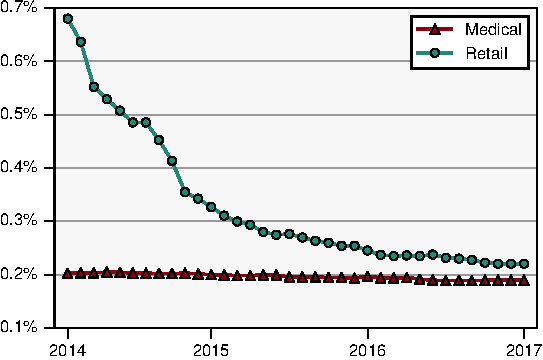
\includegraphics[scale=0.75]{images/market_share.pdf}

The 10 Commandments of Forecasting
\vspace{1\baselineskip}

{\scriptsize Silvia, J, Iqbal, A, et. al (2014), ‘Economic and Business Forecasting’.}

\vspace{1\baselineskip}

\begin{enumerate}
\item Know what you are forecasting.
\item Understand the purpose of forecasting.
\item Acknowledge the cost of the forecast error.
\item Rationalize the forecast horizon.
\item Understand the choice of variables.
\item Rationalize the forecasting model used.
\item Know how to present the results.
\item Know how to decipher the forecast results.
\item Use recursive methods.
\item Understand that forecasting models evolve over time.
\end{enumerate}
\end{frame}


\begin{frame}{}
The out-of-sample root mean square error (RMSE) can quantify forecast error.

$$
RMSE = \sqrt{\frac{1}{T}\Sigma(Y_{t+1} - \hat{Y}_{t+1})^2}
$$
\end{frame}

\section{Application}

% 1.
\begin{frame}{1. Know what you are forecasting}
\begin{itemize}
\item Forecast total sales and total plants grown in Massachusetts in 2021 and 2022 to compare the historic and estimated growth.
\end{itemize}
\end{frame}

% 2.
\begin{frame}{2. Understand the purpose of forecasting}
\begin{itemize}
\item Get better expectations for the size and growth rate of the Massachusetts cannabis industry in 2021 and 2022.
\end{itemize}
\end{frame}

% 3.
\begin{frame}{3. Acknowledge the cost of the forecast error.}
\begin{itemize}
\item Overstating growth may lead to foolhardy decisions, where as understating growth may leave money on the table.
\end{itemize}
\end{frame}

% 4.
\begin{frame}{4. Rationalize the forecast horizon}
\begin{itemize}
\item Forecasting a series for 2021 is a long, yet informative horizon. A shorter time frame may be less informative and a longer time frame may yield unreliable forecasts.
\end{itemize}
\end{frame}

% 5.
\begin{frame}{5. Understand the choice of variables.}
\begin{itemize}
\item Historic plant totals and cannabis sales in Massachusetts from November 2018 through October 2021 will be used, utilizing all of the available data under the principle to never throw away data.
\end{itemize}
\end{frame}

% 6.
\begin{frame}{6. Rationalize the forecasting model used.}
\begin{itemize}
\item An atheoretical forecasting approach, Box-Jenkins methodology, will be utilized. The Box-Jenkins methodology is useful for short-term forecasting, but less useful for long-term forecasting because the model may not capture slower moving variables that define the state of the economy.

\vspace{\baselineskip}
AR(p) process:
$$
y_t = \alpha + \beta_1 y_{t-1} + \beta_2 y_{t-2} + ... + \beta_p y_{t-p} + \epsilon_t
$$
MA(q) process:
$$
y_t = \theta + \gamma_1 \epsilon_{t-1} + \gamma_2 \epsilon_{t-2} + ... + \gamma_q \epsilon_{t-q} + \epsilon_t
$$
\end{itemize}
\end{frame}

% 7.
\begin{frame}{7. Know how to present the results.}
\begin{itemize}
\item Always show the data (in this case in a figure).
\end{itemize}
\end{frame}

% 8.
\begin{frame}{8. Know how to decipher the forecast results.}
\begin{itemize}
\item Look for seasonality, etc.
\end{itemize}
\end{frame}

% 9.
\begin{frame}{9. Use recursive methods.}
\begin{itemize}
\item When future data is released, calculate the RMSE for actual forecasts and create new forecasts.
\end{itemize}
\end{frame}

% 10.
\begin{frame}{10. Understand that forecasting models evolve over time.}
\begin{itemize}
\item See if better forecasting models predict better.
\end{itemize}
\end{frame}


%------------------------------------------------------------------%
% Takeaway
%------------------------------------------------------------------%

\begin{frame}{}
\begin{center}
\begin{minipage}{3.85in}
Thank you for coming.
\end{minipage}
\end{center}
\end{frame}

%------------------------------------------------------------------%
\end{document}
%------------------------------------------------------------------%